% Copyright (C) 2019 BARBOTIN Nicolas
\documentclass[a4paper,12pt]{article}

\usepackage[french]{babel}
\usepackage[T1]{fontenc}
\usepackage[utf8]{inputenc}
\usepackage[sfdefault]{roboto}
\usepackage{courier}
\usepackage{fullpage}
\usepackage{fancyhdr}
\usepackage{lastpage}
\usepackage{xcolor}
\usepackage{float}
\usepackage{titling}
\usepackage{tikz}
\usepackage{listings}
\usepackage{glslListings}
\usepackage{calc}
\usepackage[compact]{titlesec}
\usepackage{graphicx} %\usepackage{subfig} %%Subfigures inside a figure
%\usepackage{setspace}

%% Math Packages
\usepackage{amsmath}
\usepackage{amsthm}
\usepackage{amsfonts}
\usepackage{stmaryrd}

%% Document properties
\title{IN55 -- Rapport de projet}
\author{A. Einholtz et N. Barbotin}

%% PDF Meta
\usepackage[pdftex,
            pdfauthor={\theauthor},
            pdftitle={\thetitle}]{hyperref}

%% Line Spacing
%\singlespacing        %% 1-spacing (default)
%\onehalfspacing       %% 1,5-spacing
%\doublespacing        %% 2-spacing

%% Custom Colors
\definecolor{dgray}{gray}{0.25}
\definecolor{dgreen}{rgb}{0,0.5,0}
\definecolor{preprocessor}{rgb}{0.5,0.25,0}
\definecolor{glslType}{rgb}{0.5,0,1}


%% Page style
\pagestyle{fancy}
\renewcommand{\headrulewidth}{0pt}
\fancyhead{}
\fancyfoot[L]{\fontsize{11pt}{11pt}\selectfont\textcolor{dgray}{\theauthor}}
\fancyfoot[C]{} %\fancyfoot[C]{\fontsize{11pt}{11pt}\selectfont\textcolor{dgray}{\thetitle}} % Broken by titlesec ?!
\fancyfoot[R]{\fontsize{11pt}{11pt}\selectfont\textcolor{dgray}{Page \thepage\ sur \pageref*{LastPage}}}

%% Custom Math Operators
\DeclareMathOperator{\sinc}{sinc}

%% Custom commands
\newcommand*\circled[1]{\tikz[baseline=(char.base)]{
            \node[shape=circle,draw,inner sep=0.25pt] (char)
            {\rule[-3pt]{0pt}{\dimexpr2ex}#1};}}

\newcommand{\svg}[2][0cm]{
    \begin{figure}[H]
        \centering
        \def\svgwidth{\columnwidth - #1}
        \input{#2.pdf_tex}
    \end{figure}
}

\newcommand{\shadersrc}[1]{
    \lstinputlisting[language=GLSL]{../shaders/#1}
}

\newcommand{\abs}[1]{\left\lvert #1 \right\rvert}
\newcommand{\norm}[1]{\left\lVert#1\right\rVert}

%% Language styles
\lstset{language=GLSL,
        basicstyle=\ttfamily,
        keywordstyle=[1]\color{glslType}\ttfamily,
        keywordstyle=[2]\color{blue}\ttfamily,
        keywordstyle=[3]\color{blue}\ttfamily,
        keywordstyle=[4]\color{preprocessor}\ttfamily,
        stringstyle=\color{red}\ttfamily,
        commentstyle=\color{dgreen}\ttfamily,
        showstringspaces=false,
        frame=single,
        rulecolor=\color{gray},
        aboveskip=8pt,
        belowskip=0pt,
        breaklines=true,
        postbreak=\mbox{\textcolor{red}{$\hookrightarrow$}\space}
}

%%%%%%%%%%%%%%%%%%%%%%%%%%%%%%%%%%%%%%%%%%%%%%%%%%%%%%%%%%%%%%%%%%%%%%%%%%%%%%%%%%%%%%%%%%%%%%%%%%%%%%%%%%%%%%%%%%%%%%%%%%
%% DOCUMENT
\begin{document}
\setlength{\parindent}{0cm}
\setlength{\parskip}{8pt}

\begin{center}
    % Title
    \Huge\thetitle

    \vfill
    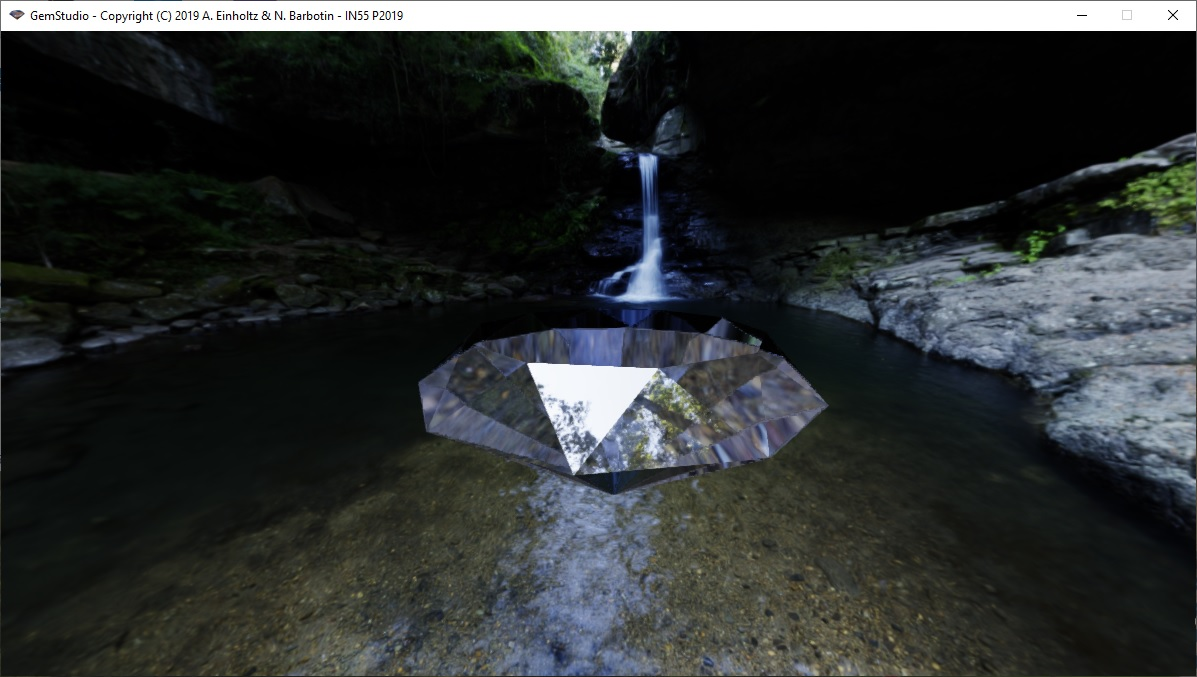
\includegraphics[width=15cm]{screenshot.jpg}
    \vfill
\end{center}

\newpage
\tableofcontents

\newpage
\section{Introduction}
\subsection{Présentation du projet}
Dans le cadre de l'UV IN55 lors du semestre de printemps 2019, nous avons été chargé de réaliser
un projet basé sur OpenGL. Le sujet que nous avons sélectionné visait à faire le rendu de pierres
précieuses en temps réel. Pour cela, nous avons utilisé C++ avec les bibliothèques GLFW pour la
gestion de la fenêtre et GLEW pour le chargement d'OpenGL. Les mathématiques et l'interface graphique
sont gérées par des bibliothèques maisons, soit MGPCL et AISO.

\subsection{Utilisation}
Lorsque \emph{GemStudio} est lancé, l'utilisateur est acueilli avec le rendu d'une gemme fond, et de
deux fênetres. La première permet de contrôler la vue et la seconde permet de modifier l'apparence de
la gemme. Ces fenêtres peuvent être fermées pour profiter de la vue, mais peuvent être réouvertes à tout
moment à l'aide des touches F1 et F2.

\subsubsection{Fenêtre de vue}
Les paramètres ajustable via cette fenêtre sont les suivant:
\begin{itemize}
    \item Champ de vision: il s'agît du FOV
    \item Vitesse d'adaption de l'exposition: permet de contrôler la vitesse à laquelle l'œuil s'adapte à la luminance de la scène
    \item Seuil de bloom: luminance à partir de laquelle l'utilisateur est considéré comme ébloui, résultant en un flou léger
    \item Vitesse de la caméra: vitesse à laquelle la caméra orbital tourne autour de la gemme
    \item Effets: permet d'activer ou de désactiver les effets utilisés pour le rendu
    \item Affichage: propose de contrôler les IPS et d'afficher des informations de débogage
    \item Changer la skybox: lorsque les environment map supplémentaires ont été téléchargées, permet de passer à l'environment map suivante
\end{itemize}

\subsubsection{Fenêtre de customisation}
Cette fenêtre permet d'ajuster l'apparence de la gemme:
\begin{itemize}
    \item Couleur: permet de changer la couleur de la gemme
    \item Indice de réfraction: permet de changer l'indice de réfraction
    \item N: nombre de côtés de la gemme
    \item H: hauteur de la partie inferieure
    \item R: rayon de l'interface inferieure/superieure
    \item dH: surélévation de la partie superieure
    \item dR: rapport entre R et le rayon de la face du haut
\end{itemize}

\subsubsection{Scène}
En plus de pouvoir changer la vitesse de la caméra, l'utilisateur peut contrôler celle-ci. En effet,
il peut utiliser (en dehors des fenêtres) la molette de sa souris pour changer l'altitude la caméra
(la distance à laquelle celle-ci orbite autour de la gemme), ainsi que la longitude et la latitude
en bougeant la souris tout en gardant le clic gauche enfoncé. Il peut aussi utiliser la touche C pour
passer de la caméra orbitale à la caméra libre, et vice-versa. Cette dernière se contrôle avec les
touches ZQSD pour la déplacer, et la souris (aussi en maintenant le clic gauche enfoncé)
pour l'orienter.

\subsection{Répartition des tâches}
Amaury s'est chargé la boucle principale, la gestion de la fenêtre, des évènements, et des objets du jeu
(dont la génération de la gemme). Nicolas s'est concentré sur les effets visuels: réfraction et réflection,
exposition automatique, etc\ldots

\subsection{Choix techniques}
Deux effets principaux interviennent dans le visuel des pierres précieuses: la réflection et la réfraction.
Ces effets étant difficile à mettre en œuvre en temps réel (c'est-à-dire, sans raytracing), nous avons décidé
de se limiter à un seul et unique objet dans toute la scène: la pierre précieuse. Celle-ci est placée dans un
décor reposant sur une \emph{environment map}; il s'agît d'une texture qui considérée comme \og à l'infini \fg
\ par rapport à la caméra. Cela permet d'accélérer de manière importante le rendu et permet d'atteindre une
centaine d'images par seconde sur une Intel HD Graphics 620, toute en gardant une qualité décente.

En plus de la réflection et de la réfraction, nous avons décidé d'implémenter les effets suivants:
\begin{itemize}
    \item Pipeline \emph{High-Dynamic Range} (HDR), pour assurer la qualité des réflections
    \item Exposition automatique: contrôle automatiquement la luminosité de la scène de manière à percevoir un maximum de couleurs différentes
    \item Bloom: effet d'éblouissement lorsque la caméra est exposée à une lumière importante
    \item Lens flare: imitation des artéfacts visuels produit par les imperfections des lentilles, perçus généralement lorsque le soleil fait directement face à la caméra
    \item Fast Approximative Anti-aliasing (FXAA) pour réduire \og l'aliasing \fg
\end{itemize}

\section{Fonctionnement}
\subsection{Classes C++}
Le projet est séparé en 10 classes principales:

\subsubsection{MainApp}
C'est elle qui gère la fenêtre, les évènements (position de la souris, entrée clavier etc\ldots), et tout le
rendu de la scène (skybox, objets du jeu, etc\ldots), et la pile de matrice modèle.
Pour ce faire, elle fait appel à toutes les autres classes décrites dans cette section. Elle gère aussi l'IHM,
mais nous avons choisi de ne pas détailler cette partie dans ce rapport.

\subsubsection{Camera, FreeCamera et RotatingCamera}
La classe Camera est une interface utilisé pour décrire une caméra; c'est-à-dire un objet capable de déterminer
la matrice de vue. En plus de cette matrice, l'interface Camera se doit de retourner un vecteur contenant la
position de la dîte caméra, et ce afin de pouvoir toujour placer le centre de la skybox en cette position.

Le projet propose deux types de caméra:
\begin{itemize}
    \item FreeCamera: la caméra libre habituelle, que l'on peut contrôler avec la souris et les touches ZQSD
    \item RotatingCamera: une caméra orbitale qui tourne toute seule autour de l'origine. L'utilisateur peut en prendre le contrôle afin d'ajuster l'alititude, la longitude et la latitude à sa guise
\end{itemize}

\subsubsection{GameObject et Gem}
GameObject est une interface représentant un objet du jeu; elle avait été crée dans l'optique de pouvoir supporter
différents objets dans une même scène, mais au final nous n'avons fait qu'un seul objet: la gemme.

La classe Gem implémente GameObject et est chargé de généré selon quelques paramètres les vertices et les indices
nécéssaire au rendu d'une gemme. 5 paramètres sont supportés lors de la génération:
\begin{itemize}
    \item Le nombre de côtés
    \item La hauteur de la partie inferieure
    \item Le rayon de la séparation inferieure/superieure
    \item La hauteur de la partie superieure
    \item Le rayon de la face du haut
\end{itemize}

La couleur peut, quand à elle, être changée via la méthode \texttt{changeColor}.

\subsubsection{Skybox}
Cette classe gère 4 choses:
\begin{itemize}
    \item Le chargement d'une environment map HDR au format RGBE
    \item La texture associée à cette environment map (pour la skybox)
    \item La cubemap associée à cette environment map (pour la réflection et la réfraction)
    \item La vertices de la skybox (c'est-à-dire, les vertices d'un cube texturé)
\end{itemize}

\ \\
Le chargement de environment map étant très long (1-5 secondes), la classe Skybox propose deux moyens de chargement:
synchrone et asynchrone. Une skybox étant nécéssaire pour faire fonctionner l'application, la première environment map
est chargée de manière synchrone au démarrage de l'application. Les suivantes sont chargée de manière asynchrone de
manière à limiter le gel de l'écran.

\subsubsection{Autres classes}
Les classes restantes sont les suivantes:
\begin{itemize}
    \item Framebuffer: une classe utilitaire pour gérer la création de Framebuffer OpenGL
    \item DownloadManager: sert à gérer le téléchargement des environment map. Celles-ci étant très lourdes (24 Mo chacunes), nous avons choisi de n'en fournir de base qu'une seule de basse qualité. Lors du premier lancement de l'application, cette classe s'occupe justement de télécharger les autres
    \item Histogram: gère tout ce qui concerne l'exposition automatique: le calcul de l'histogramme avec des \emph{compute shaders}, puis le calcul de l'exposition de la prochaine trame
\end{itemize}

\subsubsection{Diagramme de classe}
Voici le diagramme de classe résumant le tout:
\svg{UML}

\subsection{Pipeline de rendu}
Le rendu de la scène est réalisé avec la pipeline suivante:
\svg{PipelineDeRendu}

\subsubsection{Passe de rendu principale}
La passe de rendu principale est celle durant laquelle les éléments visuels principaux sont dessinés; c'est-à-dire
la \emph{skybox} et la gemme. Comme il s'agît d'une passe de rendu HDR, cette passe de rendu prends en compte
l'exposition déterminée par le système d'exposition automatique, décrit plus bas. Enfin, cette passe de rendu
génère en plus du color buffer habituel, un second buffer HDR qui sera plus tard utilisé pour le \emph{bloom}
(l'effet d'éblouissement). Ce buffer est princialement noir, sauf aux endroits où la couleur dépasse un
seuil de luminance définit par l'utilisateur. Dans ce cas, le buffer de bloom contient la même valeur que le color
buffer. Ceci se résume par le code GLSL suivant:

\begin{lstlisting}
float luma = dot(final, vec3(0.2126, 0.7152, 0.0722));

if(luma > u_BloomThreshold)
    out_Bloom = vec4(final, 1.0);
else
    out_Bloom = vec4(0.0, 0.0, 0.0, 1.0);
\end{lstlisting}

La \emph{skybox} est un simple cube texturé avec l'\emph{environment map} décrite plus haut. Normalement, les faces
de la skybox doivent être placées à une distance infinie de la caméra. Comme nous ne pouvons pas vraiment faire cela,
nous simulons cet effet en placant le centre du cube à la position de la caméra, et en désactivant l'écriture dans le buffer
de profondeur (\texttt{glDepthMask}). Ainsi, tout objet déssiné après la skybox, qu'il soit devant ou derrière
celle-ci, sera tout de même déssiné à l'écran. Puisque c'est elle qui émet la lumière de toute la scène, le dessin de
ce cube est fait sans aucun calcul d'illumination.

La gemme, en revanche, subit quelques calculs d'illumination. Les deux effets à prendre en compte sont (comme dit précédemment)
la réflexion et la réfraction:
\svg[8cm]{refraction}

On part du vectur de vue $\overrightarrow{V}$ (vecteur partant du centre de la caméra et pointant vers le fragment), du vecteur
normale $\overrightarrow{N}$ et de l'indice de réfraction $\eta_{gemme}$. On en déduit le vecteur réfléchi $\overrightarrow{R}$
et réfracté $\overrightarrow{R_2}$, avec lesquels on lit la cubemap pour trouver les couleurs correspondantes. Les deux couleurs
sont ensuite mixées ensemble selon le coefficient de fresnel. Celui-ci dépends de l'indice de réfraction et du produit scalaire
$\overrightarrow{L}\cdot\overrightarrow{H}$. Or, on constate dans notre cas que le vecteur de direction de la lumière $\overrightarrow{L}$
est égal à $-\overrightarrow{R}$ (puisque la lumière vient de l'environment map). On constate aussi que:
\[
    \overrightarrow{H} = \frac{\overrightarrow{V} + \overrightarrow{L}}{\norm{\overrightarrow{V} + \overrightarrow{L}}}
    = \frac{\overrightarrow{V} - \overrightarrow{R}}{\norm{\overrightarrow{V} - \overrightarrow{R}}}
    = \ldots = -\overrightarrow{N}
\]
Ce qui au final nous donne:
\[
    \overrightarrow{L}\cdot\overrightarrow{H} = (-\overrightarrow{R})\cdot(-\overrightarrow{N}) = \overrightarrow{R}\cdot\overrightarrow{N}
\]
Tout cela se traduit par le shader suivant:
\begin{lstlisting}
vec3 N  = normalize(f_Normal);
vec3 V  = normalize(f_WorldPos - u_CamPos);
vec3 R  = normalize(reflect(V, N));
vec3 R2 = normalize(refract(V, N, 1.0 / u_IOR));

float fresnel = computeFresnel(u_IOR, max(0.0, dot(R, N)));
vec3 diffuse  = texture(u_CubeMap, R2).rgb * f_Color.rgb;
vec3 specular = texture(u_CubeMap, R).rgb;
vec3 final    = mix(diffuse, specular, fresnel) * pow(2.0, u_Exposure);

out_Color = vec4(final, 1.0);
\end{lstlisting}

\subsubsection{Réfraction interne et passe de face arrière}
Le \emph{shading} présenté dans la section précédente est correct, mais présente un défaut important: la réfraction ne se
produit que sur la face avant. En réalité, le rayon réfracté $\overrightarrow{R_2}$ devrait continuer à l'intérieur de l'objet
avant de se \og heurter \fg\ à la face arrière, sur laquelle il est à nouveau réfléchi et réfracté. Le nouveau rayon réfléchi
risque de \og rebondir \fg\ encore quelques fois dans la pierre, et simuler cet effet serait difficile. Le nouveau rayon réfracté
en revanche sort de l'objet, et il suffit alors d'utiliser la cubemap pour trouver la bonne couleur à afficher.
\svg[6cm]{refr_int}

On cherche donc à calculer $\overrightarrow{R_2'}$. Pour cela, on réalise au préalable le rendu d'une texture de profondeur ainsi
que d'une texture de normale constitué des faces arrières (\texttt{glCullFace(GL\_FRONT)}) de la gemme. Ceci nous permettra d'obtenir
la profondeur (en espace écran) ainsi que la normale (en espace monde) de tout point sur l'écran. Le rendu de la gemme décrit précédemment
est ensuite modifié:
\begin{itemize}
    \item Passer $\overrightarrow{R_2}$ en espace écran
    \item Partir des coordonnées $\overrightarrow{P}$ du fragment en cours de calcul
    \item Ajouter $\overrightarrow{R_{2,ecran}}\times pas$ à $\overrightarrow{P}$
    \item Faire de même jusqu'à ce que $P_z \geq \mathcal{D}(P_x, P_y)$ ($\mathcal{D}$ étant la profondeur de face arrière, retrouvée à partir de la texture générée tout à l'heure)
    \item A cette étape, on dispose des coordonnées espace écran de l'intersection entre $\overrightarrow{R_2}$ et la face arrière
    \item Retrouver $\overrightarrow{N'} = -\overrightarrow{\mathcal{N}}(P_x, P_y)$ avec $\mathcal{N}$ la normale de face arrière
    \item Calculer $\overrightarrow{R_2'}$ avec $\overrightarrow{R_2}, \overrightarrow{N'}$ et l'indice de réfraction
\end{itemize}

\ \\
Reste à déterminer un pas convenable de manière à ne pas sauter trop de pixels (et perdre de la précision) et ne pas être
trop gourmand en ressources, mais le résultat est convaiquant:
\begin{figure}[H]
    \centering
    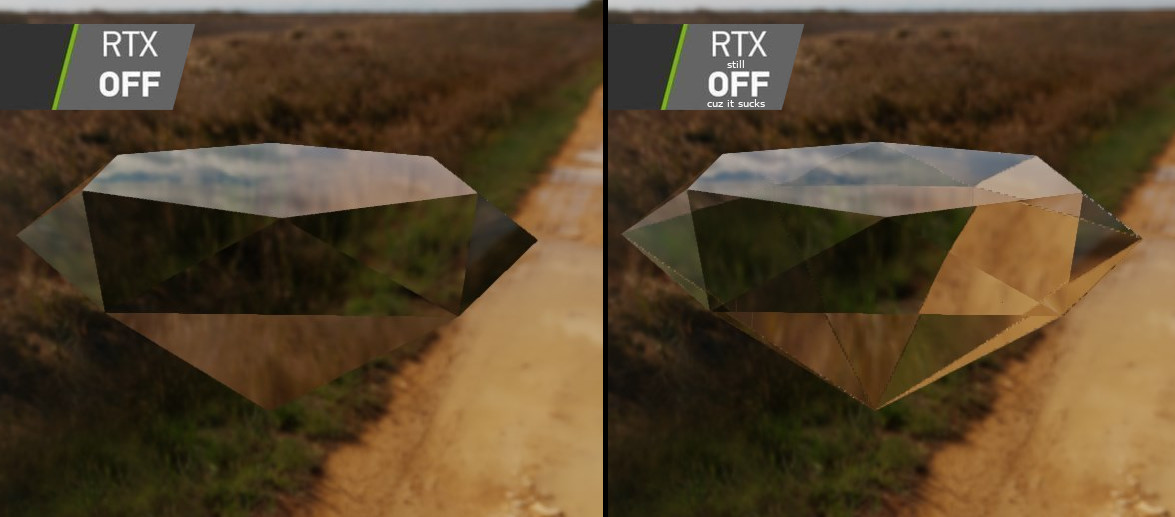
\includegraphics[width=14cm]{intref_cmp.jpg}
\end{figure}

\subsubsection{Bloom}
Le bloom se calcule avec 3 passes de rendu. La première prends en entrée la texture de bloom HDR générée par la passe de rendu princpale,
et en génère une version basse résolution. La seconde réalise un flou gaussien 12 prises horizontal, et le second un même flou mais cette
fois sur l'axe vertical. Le résultat est ensuite combiné à la couleur HDR via la passe de tone mapping.

\subsubsection{Tone mapping et anti-aliasing}
Il s'agît maintenant de convertir les couleurs HDR en couleurs LDR ($\mathbb{R}_+^3 \to [0; 1]^3$), affichable à l'écran.
Pour cela, on utilise un \emph{tone mapping}. Il existe une multitude de tone mapping, chacun adapté à une scène différente.
Le meilleur tone mapping est celui ajusté par un artiste spécifiquement pour la scène; mais comme aucun de nous n'a fait les
beaux-arts, nous avons juste implémenté un tone mapping sous le nom de \emph{ACES Filmic Tone Mapping}, trouvée sur le blog de \emph{Krzysztof Narkowicz}.

La dernière étape de rendu est une passe d'anti-aliasing. En l'occurrence il s'agît de FXAA, \emph{Fast Approximative Anti-Aliasing}.
C'est un anti-aliasing très basique sous forme de filtre. Il produit un faible flou au niveau des bords, mais est néanmoins très rapide.

\subsubsection{Exposition automatique}
L'exposition automatique permet d'ajuster l'exposition de la scène de manière à maximiser les détails affichés à l'écran. Si la scène
est sous-exposée, les endroits un peu sombre apparaîtrons noir. Si elle est sur-exposée, les endroits bien éclairés seront trop blanc
pour y distinguer quelque-chose. Lorsque la scène présente à la fois des zones sombres et claires (par exemple: salle sombre avec fenêtre
qui donne vers l'exterieur), il faut choisir la bonne exposition. Cela se fait instinctivement pour un humain. Dans un rendu 3D, en revanche,
cela requiert un peu de calcul. Voici la manière dont nous procédons:
\begin{itemize}
    \item On calcul un histogramme d'indice de lumination à partir du rendu actuel
    \item On enlève un pourcentage des pixels les plus lumineux
    \item On enlève un pourcentage des pixels les plus sombres
    \item On calcul la luminance moyenne de ce qu'il reste
    \item On en déduit une nouvelle exposition pour la trame suivante
    \item Pour éviter les changements brusques, et pour simuler le changement progressif de l'œuil, on fait varier en exponentielle inverse l'exposition
\end{itemize}

\section{Conclusion}
A travers ce projet nous avons pu répondre à la problématique de génération et rendu d'une
pierre précieuse en temps réel, et ce en utilisant OpenGL. Ce projet nous aura permis bien
évidemment de s'accomoder avec cette bibliothèque graphique, mais aussi d'en apprendre beacoup
sur la synthèse d'image photoréaliste de par les différents effets que nous avons pu implémenter.

\subsection{Limites et améliorations possibles}
Notre projet pourrait cependant être amélioré, notamment sur les points suivants:
\begin{itemize}
    \item Implémenter "real time rendering of refraction of nearby objects" pour pouvoir dessiner plusieurs objets
    \item Accélérer la recherche de profondeur dans le shader de la gemme en utilisant un algorithme de recherche dichotomique
    \item Utiliser des couleurs sRGB
    \item Implémenter un meilleur anti-aliasing (par exemple Temporal Anti-Aliasing, très efficace et très à la mode en ce moment)
    \item Plusieurs rebonds dans le shader de la gemme
\end{itemize}

\subsection{Bibliographie}
(A compléter avec les bons liens et les ISBN)
\begin{itemize}
    \item \emph{Mathematics for 3D Game Programming and Computer Graphics, Third Edition}
    \item ACES Filmic Tone Mapping
    \item Automatic Exposure
\end{itemize}

\end{document}
